\FloatBarrier

\begin{figure}[h!]
	\centering
	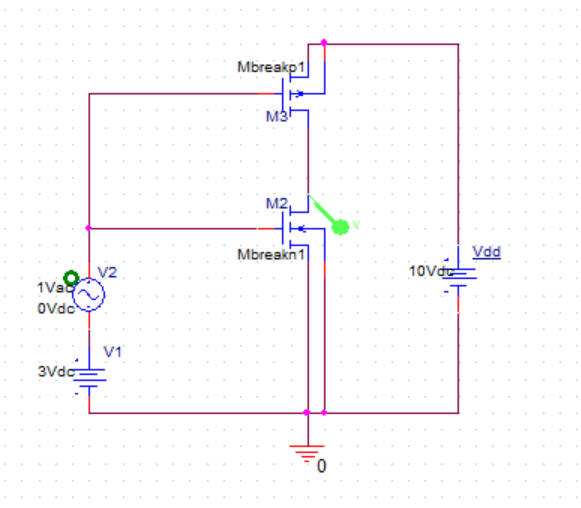
\includegraphics[scale=0.75]{./images/circuit4.PNG}
	\caption{CMOS Amplifier}
	\label{fig:circuit4}
\end{figure}

\FloatBarrier

\FloatBarrier

\begin{figure}[h!]
	\centering
	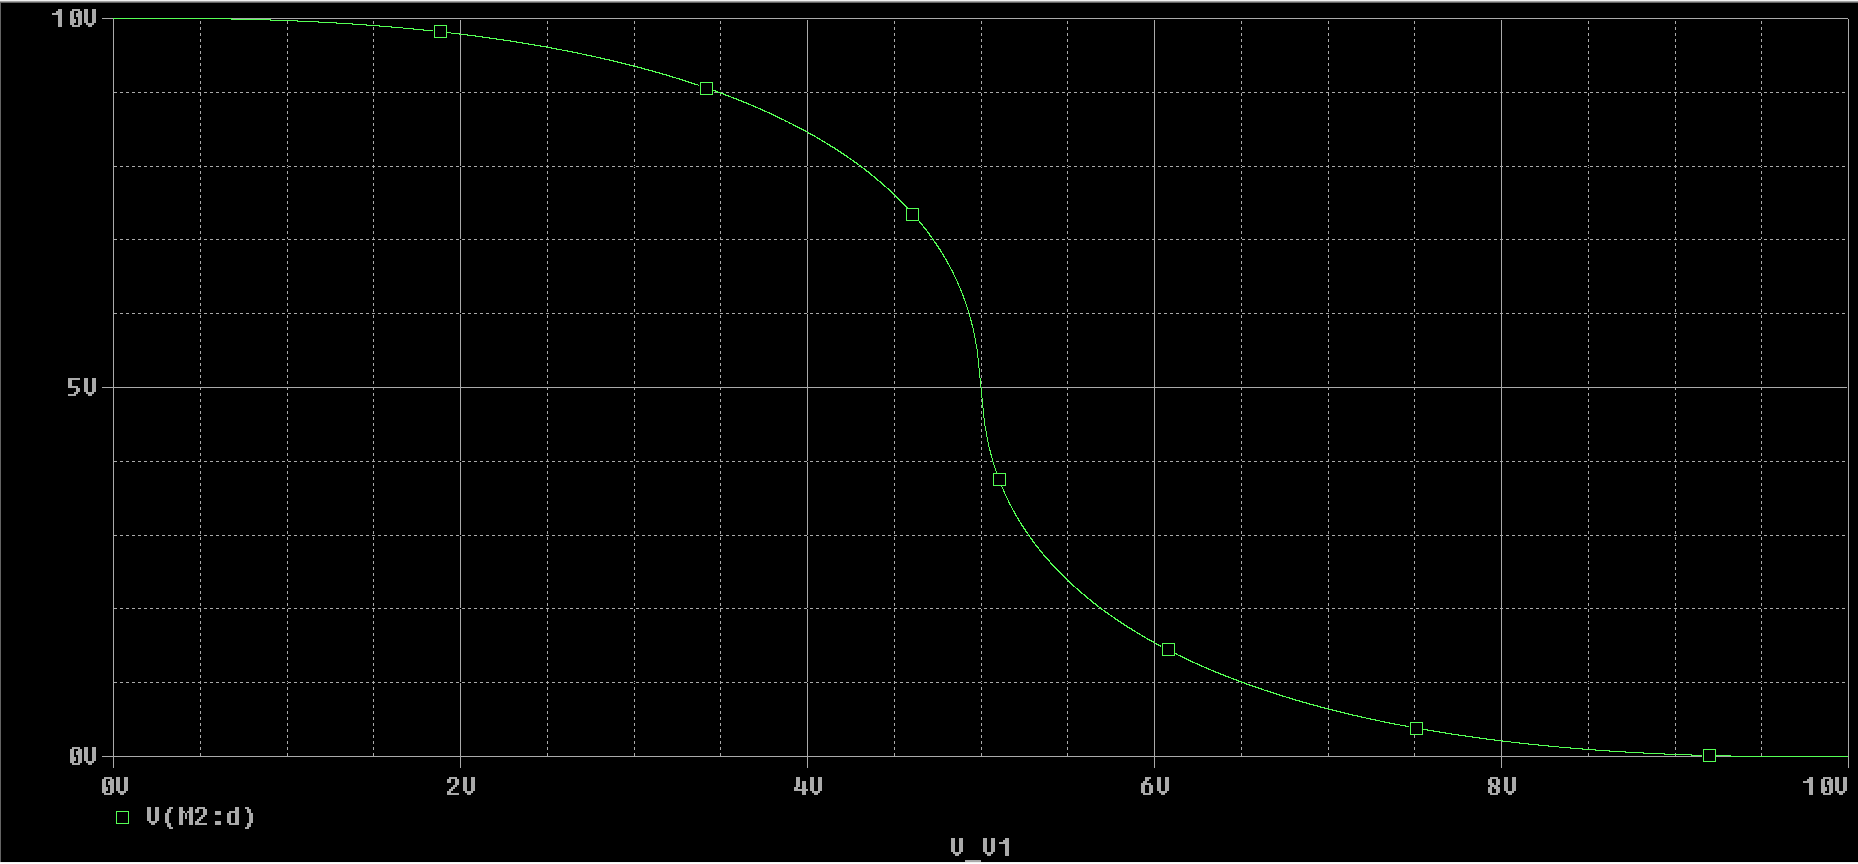
\includegraphics[scale=0.50]{./images/dc_sweep_vout_vs_vgs.PNG}
	\caption{Voltage Transfer Characteristic}
	\label{fig:dc_sweep_vout_vs_vgs}
\end{figure}

\FloatBarrier

% How does Vout change with biasing?
The CMOS amplifier has a sharper decrease than when only NMOS transistors are used. However, the descent is not as sharp as when a resistor is used, except possibly at $V_{GS} = 5$\si{\volt}. In order for the amplifier to minimize distortions in the output waveform, the bias point should be close to $5$\si{\volt}. However, the input signal must be very small, or the amplifier quickly exhibits nonlinear behavior. However, very good linearity is achieved near a $5$\si{\volt} bias point. Also, like with the other common source amplifiers, increasing the input bias voltage decreases the output bias voltage.
